\documentclass{article}
\usepackage{nips07submit_e,times}
\usepackage{graphicx}
%\documentstyle[nips07submit_09,times]{article}

\title{Review of Probability Theory}


\author{
Arian Maleki \\
Department of Electrical Engineering\\
Stanford University\\
Stanford, CA 94305 \\
\texttt{arianm@stanford.edu} \\
}

% The \author macro works with any number of authors. There are two commands
% used to separate the names and addresses of multiple authors: \And and \AND.
%
% Using \And between authors leaves it to \LaTeX{} to determine where to break
% the lines. Using \AND forces a linebreak at that point. So, if \LaTeX{}
% puts 3 of 4 authors names on the first line, and the last on the second
% line, try using \AND instead of \And before the third author name.
\usepackage{amssymb}
\usepackage{graphicx}
\usepackage{amsmath}
\usepackage{color}
\usepackage{dsfont}
\usepackage{amsthm}

\DeclareMathOperator*{\argmax}{arg\,min}

\newtheorem{thm}{Theorem}[section]
\newtheorem*{definition}{Definition}
\newtheorem{cor}[thm]{Corollary}
\newtheorem{lem}[thm]{Lemma}
\begin{document}

\makeanontitle

Probability theory is the study of uncertainty.  Through this class, we will be relying on concepts from probability
theory for deriving machine learning algorithms.  These notes attempt to cover the basics of probability theory at a
level appropriate for CS 229.  The mathematical theory of probability is very sophisticated, and
delves into a branch of analysis known as \textbf{measure theory}.  In
these notes, we provide a basic treatment of probability that does
not address these finer details.  

\section{Elements of probability}

In order to define a probability on a set we need a few basic elements,
\begin{itemize}
\item \textbf{Sample space} $\Omega$: The set of all the outcomes of a random
  experiment.  Here, each outcome $\omega \in \Omega$ can be thought
  of as a complete description of the state of the real world at the
  end of the experiment.
\item \textbf{Set of events} (or \textbf{event space}) $\mathcal{F}$: 
  A set whose
  elements $A \in \mathcal{F}$ (called \textbf{events}) are subsets of $\Omega$
  (i.e., $A \subseteq \Omega$ is a collection of possible outcomes of an
  experiment).\footnote{
  $\mathcal{F}$ should satisfy three properties: 
  (1) $\emptyset \in \mathcal{F}$;
  (2) $A \in \mathcal{F} \Longrightarrow \Omega \setminus A \in \mathcal{F}$; and
  (3) $A_1, A_2 , \ldots \in \mathcal{F} \Longrightarrow \cup_i A_i \in \mathcal{F}$.
}.
\item \textbf{Probability measure}: A function $P : \mathcal{F} \rightarrow \mathbb{R}$ that satisfies the following properties,
       \begin{description}
          \item[-] $P(A) \geq 0$, for all $A \in \mathcal{F}$
          \item[-] $P(\Omega)=1$
          \item[-] If $A_1,A_2, \ldots$ are disjoint events (i.e., $A_i \cap A_j= \emptyset$ whenever $i \neq j$), then
          \begin{equation*}
            P(\cup_{i} A_i)= \sum_i P(A_i)
          \end{equation*}
        \end{description}
\end{itemize}
These three properties are called the \textbf{Axioms of Probability}.

\textbf{Example}: Consider the event of tossing a six-sided die. The
sample space is $\Omega= \{1,2,3,4,5,6\}$. We can define different
  event spaces on this sample space. For example, the simplest event
  space is the trivial event space $\mathcal{F}=\{\emptyset,
  \Omega\}$. Another event space is the set of all subsets of
  $\Omega$. For the first event space, the unique probability measure 
  satisfying the requirements above is
  given by $P(\emptyset)=0, P(\Omega)=1$. For the second event space,
  one valid probability measure is to assign the probability of each set in the event space to be $\frac{i}{6}$
  where $i$ is the number of elements of that set; for example,
  $P(\{1,2,3,4\})= \frac{4}{6}$ and $P(\{1,2,3\})= \frac{3}{6}$. \\

\textbf{Properties}:
\begin{description}
\item[-] {If $ {A \subseteq B \Longrightarrow P(A) \leq P(B)}$.}
\item[-] ${P(A \cap B) \leq \min(P(A), P(B))}$.
\item[-] (Union Bound) ${P(A \cup B) \leq P(A)+P(B)}$.
\item[-] ${P(\Omega \setminus A)=1-P(A)}$.
\item[-] {(Law of Total Probability) If $A_1,\ldots,A_k$ are a set of disjoint events such that $\cup_{i=1}^k A_i = \Omega$, then $\sum_{i=1}^k P(A_k) = 1$.}
\end{description}

\subsection{Conditional probability and independence}

Let $B$ be an event with non-zero probability. The conditional probability of any event $A$ given $B$ is defined as,
\begin{equation*}
P(A | B)\triangleq \frac{P(A \cap B)}{P(B)}
\end{equation*}
In other words, $P(A| B)$ is the probability measure of the event $A$
after observing the occurrence of event $B$. Two events are called
independent if and only if $P(A \cap B)= P(A)P(B)$ (or equivalently, $P(A|B)=P(A)$).  Therefore,
independence is equivalent to saying that observing $B$ does not have
any effect on the probability of $A$.

\section{Random variables}

Consider an experiment in which we flip 10 coins, and we want to know the
number of coins that come up heads.  Here, the elements of the sample
space $\Omega$ are 10-length sequences of heads and tails.  For example,
we might have $w_0 = \langle H, H, T, H, T, H, H, T, T, T \rangle \in
\Omega$.  However, in practice, we usually do not care about the
probability of obtaining any particular sequence of heads and tails.
Instead we usually care about real-valued functions of outcomes, such as the
number of heads that appear among our 10 tosses, or the
length of the longest run of tails.  These functions, under some
technical conditions, are known as \textbf{random variables}.

More formally, a random variable $X$ is a function $X:\Omega
\longrightarrow \mathbb{R}$.\footnote{ Technically speaking, not every
  function is not acceptable as a random variable.  From a
  measure-theoretic perspective, random variables must be
  Borel-measurable functions.  Intuitively, this restriction ensures
  that given a random variable and its underlying outcome space, one
  can implicitly define the each of the events of the event space as
  being sets of outcomes $\omega \in \Omega$ for which $X(\omega)$
  satisfies some property (e.g., the event $\{\omega : X(\omega) \ge 3 \}$).
} Typically, we will denote random
variables using upper case letters $X(\omega)$ or more simply $X$
(where the dependence on the random outcome $\omega$ is implied).  We
will denote the value that a random variable may take on using lower
case letters $x$.

\textbf{Example}: In our experiment above, suppose that $X(\omega)$ is
the number of heads which occur in the sequence of tosses $\omega$.
Given that only 10 coins are tossed, $X(\omega)$ can take only a
finite number of values, so it is known as a \textbf{discrete random
variable}. Here, the probability of the set associated with a random
variable $X$ taking on some specific value $k$ is
\begin{eqnarray*}
  P(X = k) := P(\{\omega : X(\omega) = k\}).
\end{eqnarray*}

\textbf{Example}: Suppose that $X(\omega)$ is a random variable
indicating the amount of time it takes for a radioactive particle to
decay.  In this case, $X(\omega)$ takes on a infinite number of
possible values, so it is called a \textbf{continuous random
variable}.  We denote the probability that $X$ takes on a value between 
two real constants $a$ and $b$ (where $a < b$) as 
\begin{eqnarray*}
  P(a \le X \le b) := P(\{\omega : a \le X(\omega) \le b\}).
\end{eqnarray*}

\subsection{Cumulative distribution functions}

In order to specify the probability measures used when dealing with
random variables, it is often convenient to specify alternative
functions (CDFs, PDFs, and PMFs) from which the probability measure
governing an experiment immediately follows.  In this section and the
next two sections, we describe each of these types of functions in
turn.

A \textbf{cumulative distribution function (CDF)} is a function $F_X:\mathbb{R} \rightarrow [0,1]$ which specifies a probability measure as,
\begin{equation}
F_X(x) \triangleq P(X \leq x).
\end{equation}
By using this function one can calculate the probability of any event in $\mathcal{F}$.\footnote{This is a remarkable fact and is actually a theorem that is proved in more advanced courses.} %How? First of all they define a $\pi$-system. $\mathcal{P}$ is a $\pi$-system, if $I,J \in \mathcal{P} \Longrightarrow I \cap J \in \mathcal{P}$. Then there is a theorem that says that if two probability measures are equal on a $\pi$-system then they are equal to each other on the $\sigma$-algebra generated by that $\pi$-system. Now the set of [-\infty, a] generates the Borel sigma algebra and is a $\pi$-system and therefore defines the probability uniquely!!!
Figure \ref{fig1} shows a sample CDF function.

\textbf{Properties}:
\begin{description}
\item[-] $0 \leq F_X(x) \leq 1$.
\item[-] $\lim_{x \rightarrow -\infty} F_X(x)=0$.
\item[-] $\lim_{x \rightarrow \infty} F_X(x)=1$.
\item[-] $x \leq y \Longrightarrow F_X(x)\leq F_X(y)$.
\end{description}

\begin{figure}
\begin{center}
  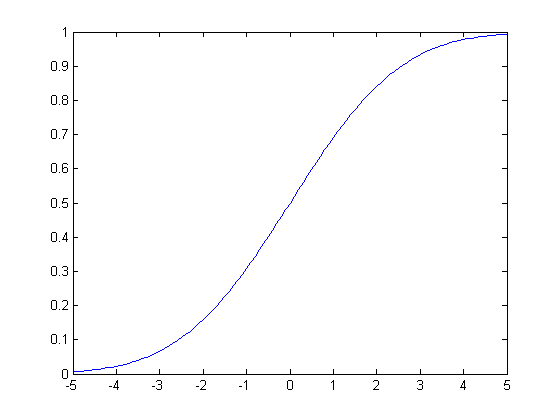
\includegraphics[width=7cm]{fig1}\\
  \caption{A cumulative distribution function (CDF).}\label{fig1}
\end{center}
\end{figure}

\subsection{Probability mass functions}

When a random variable $X$ takes on a finite set of possible values (i.e., $X$ is a discrete random variable), a simpler way to represent the probability measure associated with
a random variable is to directly specify the probability of each value that the random variable can assume.  In particular, a \emph{probability
mass function (PMF)} is a function $p_X : \Omega \rightarrow \mathbb{R}$ such that
\begin{align*}
p_X(x)\triangleq P(X=x).
\end{align*}
In the case of discrete random variable, we use the notation $Val(X)$ for the set of possible values that the random variable $X$ may assume.  For example, if $X(\omega)$ is a random
variable indicating the number of heads out of ten tosses of coin, then $Val(X) = \{0,1,2,\ldots,10\}$.  

\textbf{Properties}:
\begin{description}
\item [-] $0 \leq p_X(x) \leq  1$.
\item [-] $\sum_{x \in Val(X)} p_X(x)=1$.
\item [-] $\sum_{x \in A} p_X(x) = P(X \in A)$.
\end{description}

\subsection{Probability density functions}

For some continuous random variables, the cumulative distribution function $F_X(x)$ is differentiable everywhere.  In these cases, we define the \textbf{Probability Density Function} or \textbf{PDF} 
as the derivative of the CDF, i.e.,
\begin{equation}
f_X(x)\triangleq \frac{dF_X(x)}{dx}.
\end{equation}
Note here, that the PDF for a continuous random variable may not always exist (i.e., if $F_X(x)$ is not differentiable everywhere).

According to the properties of differentiation, for very small $\Delta x$,
\begin{equation}
P(x \leq X \leq x+ \Delta x) \approx f_X(x)\Delta x.
\end{equation}
Both CDFs and PDFs (when they exist!) can be used for
calculating the probabilities of different events. But it should be
emphasized that the value of PDF at any given point $x$ is not the probability of
that event, i.e., $f_X(x) \neq P(X = x)$.  For example, $f_X(x)$ can take on
values larger than one (but the integral of $f_X(x)$ over any subset of $\mathbb{R}$ will
be at most one).

\textbf{Properties}:
\begin{description}
\item [-] $\small{f_X(x) \geq 0}$ .
\item [-] $\small {\int_{-\infty}^\infty f_X(x) =1}$.
\item [-] $\int_{x \in A} f_X(x) dx = P(X \in A)$.
\end{description}

\subsection{Expectation}
Suppose that $X$ is a discrete random variable with PMF $p_X(x)$ and $g: \mathbb{R} \longrightarrow \mathbb{R}$ is an arbitrary function. In this case,
$g(X)$ can be considered a random variable, and we define the \textbf{expectation} or \textbf{expected value} of $g(X)$ as
\begin{align*}
E[g(X)] \triangleq \sum_{x \in Val(X)} g(x) p_X(x).
\end{align*}
If $X$ is a continuous random variable with PDF $f_X(x)$, then the expected value of $g(X)$ is defined as,
\begin{align*}
E[g(X)]\triangleq \int_{-\infty}^{\infty} g(x) f_X(x) dx.
\end{align*}
Intuitively, the expectation of $g(X)$ can be thought of as a ``weighted average'' of
the values that $g(x)$ can taken on for different values of $x$, where the weights are
given by $p_X(x)$ or $f_X(x)$.
As a special case of the above, note that the expectation, $E[X]$ of a random variable itself
is found by letting $g(x) = x$; this is also known as the \textbf{mean} of the random variable $X$.

\textbf{Properties}:
\begin{description}
\item[-] $E[a] = a$ for any constant $a \in \mathbb{R}$.
\item[-] $E[af(X)] = aE[f(X)]$ for any constant $a \in \mathbb{R}$.
\item[-] (Linearity of Expectation) $E[f(X) + g(X)] = E[f(X)] + E[g(X)]$.
\item[-] For a discrete random variable $X$, $E[1\{X = k \}] = P(X = k)$.
\end{description}

\subsection{Variance}

The \textbf{variance} of a random variable $X$ is a measure of how concentrated the distribution of a random variable $X$
is around its mean.  Formally, the variance of a random variable $X$ is defined as
\begin{align*}
  Var[X] \triangleq E[(X-E(X))^2]
\end{align*}
Using the properties in the previous section, we can derive an alternate expression for the variance:
\begin{eqnarray*}
  E[(X - E[X])^2] &=& E[X^2 - 2E[X] X + E[X]^2] \\ &=& E[X^2] - 2 E[X] E[X] + E[X]^2 \\ &=& E[X^2] - E[X]^2,
\end{eqnarray*}
where the second equality follows from linearity of expectations and the fact that $E[X]$ is actually a constant with
respect to the outer expectation.  

\textbf{Properties}:
\begin{description}
\item[-] $Var[a] = 0$ for any constant $a \in \mathbb{R}$.
\item[-] $Var[a f(X)] = a^2 Var[f(X)]$ for any constant $a \in \mathbb{R}$.
\end{description}

\textbf{Example} Calculate the mean and the variance of the uniform random variable $X$ with PDF $f_X(x)=1, \ \ \forall x \in [0,1]$, 0 elsewhere.
\begin{align*}
E[X]= \int_{-\infty}^{\infty} xf_X(x) dx= \int_{0}^{1}xdx=\frac{1}{2}. \nonumber
\end{align*}
\begin{align*}
E[X^2]=\int_{-\infty}^{\infty} x^2f_X(x) dx= \int_{0}^{1}x^2dx=\frac{1}{3}. \nonumber
\end{align*}
\begin{align*} 
Var[X]=E[X^2]-E[X]^2= \frac{1}{3}- \frac{1}{4}=\frac{1}{12}. \nonumber
\end{align*}

\textbf{Example:} Suppose that $g(x)= 1\{x \in A\}$ for some subset $A \subseteq \Omega$.
What is $E[g(X)]$? 

Discrete case: 
\begin{align*}
  E[g(X)]= \sum_{x \in Val(X)} 1\{x \in A\} P_X(x)dx= \sum_{x \in A} P_X(x)dx= P(x \in A). \nonumber
\end{align*}
Continuous case: 
\begin{align*}
  E[g(X)]= \int_{-\infty}^{\infty} 1\{x \in A\} f_X(x)dx= \int_{x \in A} f_X(x)dx= P(x \in A). \nonumber
\end{align*}

\subsection{Some common random variables}

\textbf{Discrete random variables}
\begin{itemize}
\item $X \sim Bernoulli(p)$ (where $0 \le p \le 1$): one if a coin with heads probability $p$ comes up heads, zero otherwise.
  \begin{eqnarray*}
    p(x) = \begin{cases}
      p & \text{if $p = 1$} \\
      1-p & \text{if $p = 0$}
    \end{cases}
  \end{eqnarray*}
\item $X \sim Binomial(n, p)$ (where $0 \le p \le 1$): the number of heads in $n$ independent flips of a coin with heads probability $p$.
  \begin{eqnarray*}
    p(x) = {n \choose x} p^x(1-p)^{n-x}
  \end{eqnarray*}
\item $X \sim Geometric(p)$ (where $p > 0$): the number of flips of a coin with heads probability $p$ until the first heads.
  \begin{eqnarray*}
    p(x) = p(1 - p)^{x-1}
  \end{eqnarray*}
\item $X \sim Poisson(\lambda)$ (where $\lambda > 0$): a probability distribution over the nonnegative integers used for modeling the
  frequency of rare events.
  \begin{eqnarray*}
    p(x) = e^{-\lambda} \frac{\lambda^x}{x!}
  \end{eqnarray*}
\end{itemize}

\textbf{Continuous random variables}
\begin{itemize}
\item $X \sim Uniform(a,b)$ (where $a < b$): equal probability density to every value between $a$ and $b$ on the real line.
  \begin{eqnarray*}
    f(x) = \begin{cases} 
      \frac{1}{b - a} & \text{if $a \le x \le b$} \\
      0 & \text{otherwise}
    \end{cases}
  \end{eqnarray*}
\item $X \sim Exponential(\lambda)$ (where $\lambda > 0$): decaying probability density over the nonnegative reals.
  \begin{eqnarray*}
    f(x) = \begin{cases}
      \lambda e^{-\lambda x} & \text{if $x \ge 0$} \\
      0 & \text{otherwise}
    \end{cases}
  \end{eqnarray*}
\item $X \sim Normal(\mu, \sigma^2)$: also known as the Gaussian distribution
  \begin{eqnarray*}
    f(x) = \frac{1}{\sqrt{2\pi} \sigma} e^{-\frac{1}{2\sigma^2} (x - \mu)^2}
  \end{eqnarray*}
\end{itemize}
The shape of the PDFs and CDFs of some of these random variables are shown in Figure \ref{fig2}.

 The following table is the summary of some of the properties of these distributions.
\begin{center}
\begin{tabular}{|l|l|l|l|l|} 
  \hline
  % after \\: \hline or \cline{col1-col2} \cline{col3-col4} ...
   Distribution & PDF or PMF & Mean & Variance \\
  \hline
  $Bernoulli(p)$ &  $\left\{   \begin{array}{ll}
                                 p, & \text{if $x=1$} \\
                                 1-p, & \text{if $x=0$.}
                               \end{array}
                             \right.$ & $p$ & $p(1-p)$\\
  \hline
  $Binomial(n,p)$ & $n \choose k$ $p^k(1-p)^{n-k}  $ for $ 0 \leq k \leq n$ & $np$ & $npq$ \\
  \hline
  $Geometric(p)$ & $p(1-p)^{k-1}$ \ \ for $k=1,2, \ldots$ & $\frac{1}{p}$ & $\frac{1-p}{p^2}$ \\
  \hline
  $Poisson(\lambda)$ & $e^{-\lambda} \lambda^x / x!$ \ \ for $k=1,2,\ldots$ & $\lambda$ & $\lambda$ \\
  \hline
  $Uniform(a,b)$ & $\frac{1}{b-a} \ \ \forall x \in (a,b)$  & $\frac{a+b}{2}$ & $\frac{(b-a)^2}{12}$ \\
  \hline
  $Gaussian(\mu,\sigma^2)$ & $\frac{1}{\sigma \sqrt{2 \pi}}e^{-\frac{(x-\mu)^2}{2\sigma^2}}$ & $\mu$ & $\sigma^2$ \\
  \hline
  $Exponential(\lambda)$ & $\lambda e^{-\lambda x} \ \ x \geq 0, \lambda >0$ & $\frac{1}{\lambda}$ & $ \frac{1}{\lambda ^2}$ \\
   \hline
\end{tabular}
\end{center}


\begin{figure}
\begin{center}
  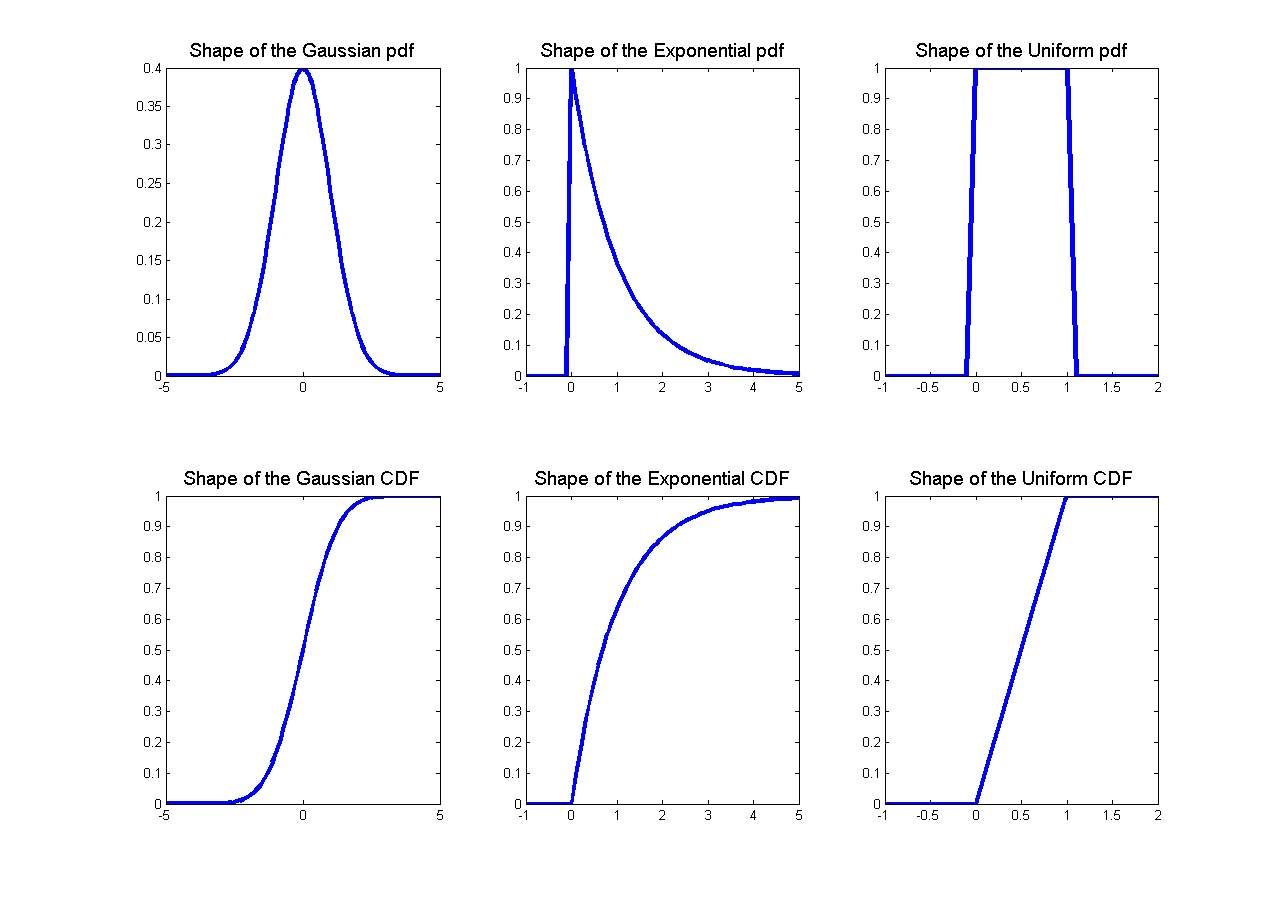
\includegraphics[width=9cm]{fig2.png}\\
  \caption{PDF and CDF of a couple of random variables.}\label{fig2}
\end{center}
\end{figure}

\section{Two random variables}

Thus far, we have considered single random variables.  In many
situations, however, there may be more than one quantity that we are
interested in knowing during a random experiment.  For instance, in an
experiment where we flip a coin ten times, we may care about both $X(\omega) =
\text{the number of heads that come up}$ as well as $Y(\omega) = \text{the
length of the longest run of consecutive heads}$.  In this section, we
consider the setting of two random variables.

\subsection{Joint and marginal distributions}

Suppose that we have two random variables $X$ and $Y$. One way to work
with these two random variables is to consider each of them
separately. If we do that we will only need $F_X(x)$ and $F_Y(y)$.
But if we want to know about the values that $X$ and $Y$ assume
simultaneously during outcomes of a random experiment, we require
a more complicated structure known as the 
\textbf{joint cumulative distribution function} of $X$ and $Y$, defined by
\begin{equation*}
F_{XY}(x,y)=P(X \leq x, Y \leq y)
\end{equation*}
It can be shown that by knowing the joint
cumulative distribution function,
the probability of any event involving $X$ and $Y$ can be calculated. 

The joint CDF $F_{XY}(x,y)$ and the joint distribution functions
$F_X(x)$ and $F_Y(y)$ of each variable separately are related by
\begin{eqnarray*}
  F_X(x) &=& \lim_{y \rightarrow \infty} F_{XY}(x,y) dy \\
  F_Y(y) &=& \lim_{x \rightarrow \infty} F_{XY}(x,y) dx.
\end{eqnarray*}
Here, we call $F_X(x)$ and $F_Y(y)$ the \textbf{marginal cumulative distribution functions}
of $F_{XY}(x,y)$.

\textbf{Properties}:
\begin{description}
\item[-] $0 \leq F_{XY}(x,y) \leq 1$.
\item[-] $\lim_{x,y \rightarrow \infty} F_{XY}(x,y)=1$.
\item[-] $\lim_{x,y \rightarrow -\infty} F_{XY}(x,y)=0$.
\item[-] $ F_X(x)= \lim_{y \rightarrow \infty} F_{XY}(x,y)$.
\end{description}

\subsection{Joint and marginal probability mass functions}

If $X$ and $Y$ are discrete random variables, then the \textbf{joint probability mass function} $p_{XY} : \mathbb{R} \times \mathbb{R} \rightarrow [0,1]$ is
defined by
\begin{eqnarray*}
  p_{XY}(x,y) = P(X = x, Y = y).
\end{eqnarray*}
Here, $0 \le p_{XY}(x,y) \le 1$ for all $x, y$, and $\sum_{x \in Val(X)} \sum_{y \in Val(Y)} p_{XY}(x,y) = 1$.

How does the joint PMF over two variables relate to the probability mass function for each variable separately? 
It turns out that
\begin{eqnarray*}
  p_X(x) = \sum_y p_{XY} (x,y).
\end{eqnarray*}
and similarly for $p_Y(y)$.  In this case, we refer to $p_X(x)$ as the
\textbf{marginal probability mass function} of $X$.  In statistics, the process of forming the
marginal distribution with respect to one variable by summing out the
other variable is often known as ``marginalization.''

\subsection{Joint and marginal probability density functions}

Let $X$ and $Y$ be two continuous random variables with joint distribution function $F_{XY}$.  In the case that
$F_{XY}(x,y)$ is everywhere differentiable in both $x$ and $y$, then we can define the \textbf{joint probability density function},
\begin{equation*}
  f_{XY}(x,y)= \frac{ \partial^2 F_{XY}(x,y)}{\partial x \partial y}.
\end{equation*}
Like in the single-dimensional case, $f_{XY}(x,y) \neq P(X = x, Y = y)$, but rather
\begin{equation*}
  \iint_{x \in A} f_{XY} (x,y) dx dy = P((X,Y) \in A).
\end{equation*}
Note that the values of the probability density function $f_{XY}(x,y)$ are always nonnegative, but they may be greater than 1.  Nonetheless, it must be the
case that $\int_{-\infty}^\infty \int_{-\infty}^\infty f_{XY}(x,y) = 1$.

Analagous to the discrete case, we define
\begin{eqnarray*}
  f_X(x) = \int_{-\infty}^{\infty}f_{XY}(x,y)dy,
\end{eqnarray*}
as the \textbf{marginal probability density function} (or \textbf{marginal
  density}) of $X$, and similarly for $f_Y(y)$.

\subsection{Conditional distributions}

Conditional distributions seek to answer the question, what is the probability distribution over $Y$, when we know
that $X$ must take on a certain value $x$?
In the discrete case, the conditional probability mass
function of $X$ given $Y$ is simply
\begin{equation*}
  p_{Y|X}(y|x) = \frac{p_{XY}(x,y)}{p_X(x)},
\end{equation*}
assuming that $p_X(x) \neq 0$.

In the continuous case, the situation is technically a little more complicated
because the probability that a continuous random variable $X$ takes on a specific value $x$ is equal to zero\footnote{
  To get around this, a more reasonable way to calculate the
  conditional CDF is,
\begin{equation*}
F_{Y|X}(y,x)= \lim_{\Delta x \rightarrow 0} P(Y \leq y | x \leq X \leq x + \Delta x).
\end{equation*}
It can be easily seen that if $F(x,y)$ is differentiable in both $x,y$ then,

\begin{equation*}
F_{Y|X}(y,x)=\int_{-\infty}^{y} \frac{f_{X,Y}(x,\alpha)}{f_X(x)}d\alpha
\end{equation*}
and therefore we define the conditional PDF of $Y$ given $X=x$ in the following way,
\begin{equation*}
f_{Y|X}(y|x)= \frac{f_{XY}(x,y)}{f_X(x)}
\end{equation*}
}.  Ignoring this technical point, we simply define, by analogy to the discrete case,
the \emph{conditional probability density} of $Y$ given $X = x$ to be 
\begin{equation*}
  f_{Y|X}(y|x) = \frac{f_{XY}(x,y)}{f_X(x)},
\end{equation*}
provided $f_X(x) \neq 0$.

\subsection{Bayes's rule}
A useful formula that often arises when trying to derive expression for the conditional probability 
of one variable given another, is \textbf{Bayes's rule}.

In the case of discrete random variables $X$ and $Y$,
\begin{equation*}
P_{Y|X}(y|x)=\frac{P_{XY}(x,y)}{P_X(x)}=\frac{P_{X|Y}(x|y)P_Y(y)}{\sum_{y' \in Val(Y)} P_{X|Y}(x|y')P_Y(y')}.
\end{equation*}

If the random variables $X$ and $Y$ are continuous,
\begin{equation*}
f_{Y|X}(y|x)=\frac{f_{XY}(x,y)}{f_X(x)}=\frac{f_{X|Y}(x|y)f_Y(y)}{\int_{-\infty}^{\infty} f_{X|Y}(x|y')f_Y(y')dy'}.
\end{equation*}

\subsection{Independence}

Two random variables $X$ and $Y$ are \textbf{independent} if $F_{XY}(x,y) = F_X(x) F_Y(y)$ for all values of 
$x$ and $y$.  Equivalently,
\begin{itemize}
\item For discrete random variables, $p_{XY}(x,y) = p_X(x) p_Y(y)$ for all $x \in Val(X)$, $y \in Val(Y)$.
\item For discrete random variables, $p_{Y|X}(y|x) = p_Y(y)$ whenever $p_X(x) \neq 0$ for all $y \in Val(Y)$.
\item For continuous random variables, $f_{XY}(x,y) = f_X(x) f_Y(y)$ for all $x,y \in \mathbb{R}$.
\item For continuous random variables, $f_{Y|X}(y|x) = f_Y(y)$ whenever $f_X(x) \neq 0$ for all $y \in \mathbb{R}$.
\end{itemize}

Informally, two random variables $X$ and $Y$ are \textbf{independent}
if ``knowing'' the value of one variable will never have any effect on
the conditional probability distribution of the other variable, that
is, you know all the information about the pair $(X,Y)$ by just
knowing $f(x)$ and $f(y)$. The following lemma formalizes this
observation:
\begin{lem}
If $X$ and $Y$ are independent then for any subsets $A, B \subseteq \mathbb{R}$, we have,
\begin{eqnarray*}
P(X \in A, Y \in B)=P(X \in A) P(Y \in B)
\end{eqnarray*}
\end{lem}
By using the above lemma one can prove that if $X$ is independent of $Y$ then any function of $X$ is independent of any function of $Y$.

\subsection{Expectation and covariance}

Suppose that we have two discrete random variables $X, Y$ and $g: \mathbf{R}^2 \longrightarrow \mathbf{R}$ is a function of these two random variables. Then the expected value of $g$ is defined in the following way,
\begin{equation*}
  E[g(X,Y)] \triangleq \sum_{x \in Val(X)} \sum_{y \in Val(Y)} g(x,y) p_{XY}(x,y).
\end{equation*}
For continuous random variables $X,Y$, the analogous expression is
\begin{equation*}
E[g(X,Y)]= \int_{-\infty}^{\infty} \int_{- \infty}^{\infty} g(x,y) f_{XY}(x,y) dxdy.
\end{equation*}

We can use the concept of expectation to study the relationship of two random variables with each other.  In particular, the \textbf{covariance} of two random variables $X$ and $Y$ is defined as
\begin{eqnarray*}
Cov[X,Y] 
&\triangleq& E[(X-E[X])(Y-E[Y])] \\
\end{eqnarray*}
Using an argument similar to that for variance, we can rewrite this as,
\begin{eqnarray*}
Cov[X,Y] 
&=& E[(X-E[X])(Y-E[Y])] \\
&=& E[XY - X E[Y] - Y E[X] + E[X] E[Y]] \\
&=& E[XY] - E[X] E[Y] - E[Y] E[X] + E[X] E[Y]] \\
&=& E[XY] - E[X] E[Y].
\end{eqnarray*}
Here, the key step in showing the equality of the two forms of covariance is in the third equality, where we use the fact that $E[X]$ and $E[Y]$ are actually constants which
can be pulled out of the expectation.  When $Cov[X,Y] = 0$, we say that $X$ and $Y$ are \textbf{uncorrelated}\footnote{
  However, this is not the same thing as stating that $X$ and $Y$ are independent!  For example, if $X \sim Uniform(-1,1)$ and $Y = X^2$, then one can show that $X$ and $Y$ are
  uncorrelated, even though they are not independent.
}.

\textbf{Properties}:
\begin{description}
\item[-] (Linearity of expectation) $E[f(X,Y) + g(X,Y)] = E[f(X,Y)] + E[g(X,Y)]$.
\item[-] $Var[X + Y] = Var[X] + Var[Y] + 2 Cov[X, Y]$.
\item[-] If $X$ and $Y$ are independent, then $Cov[X, Y] = 0$.
\item[-] If $X$ and $Y$ are independent, then $E[f(X)g(Y)] = E[f(X)] E[g(Y)]$.
\end{description}

\section{Multiple random variables}

The notions and ideas introduced in the previous section can be
generalized to more than two random variables.  In particular, suppose that we have $n$ continuous
random variables, $X_1(\omega),X_2(\omega), \ldots X_n(\omega)$.  In this section, for simplicity of presentation,
we focus only on the continuous case, but the generalization to discrete random variables works similarly.

\subsection{Basic properties}

We can define the \textbf{joint distribution function} of $X_1,X_2,\ldots,X_n$, 
the \textbf{joint probability density function} of $X_1,X_2,\ldots,X_n$, 
the \textbf{marginal probability density function} of $X_1$, and
the \textbf{conditional probability density function} of $X_1$ given $X_2,\ldots,X_n$, as

\begin{eqnarray*}
F_{X_1, X_2, \ldots, X_n}(x_1,x_2, \ldots x_n) &=& P(X_1 \leq x_1, X_2 \leq x_2, \ldots, X_n \leq x_n) \\
f_{X_1, X_2, \ldots, X_n}(x_1,x_2, \ldots x_n) &=& \frac{\partial^n F_{X_1, X_2, \ldots, X_n}(x_1,x_2, \ldots x_n)}{\partial x_1 \ldots \partial x_n} \\
f_{X_1}(X_1) &=& \int_{-\infty}^\infty \cdots \int_{-\infty}^\infty f_{X_1, X_2, \ldots, X_n}(x_1,x_2, \ldots x_n) dx_2 \ldots dx_n \\
f_{X_1 | X_2, \ldots, X_n}(x_1|x_2, \ldots x_n) &=& \frac{f_{X_1, X_2, \ldots, X_n}(x_1,x_2, \ldots x_n)}{f_{ X_2, \ldots, X_n}(x_1,x_2, \ldots x_n)}
\end{eqnarray*}

To calculate the probability of an event $A \subseteq \mathbb{R}^n$ we have,
\begin{equation}
P((x_1,x_2, \ldots x_n) \in A)= \int_{(x_1,x_2, \ldots x_n) \in A} f_{X_1,X_2,\ldots,X_n}(x_1,x_2, \ldots x_n)dx_1dx_2 \ldots dx_n
\end{equation}

\textbf{Chain rule}: From the
definition of conditional probabilities for multiple random variables, one can show that
\begin{eqnarray*}
  f(x_1,x_2,\ldots,x_n) &=& f(x_n|x_1,x_2\ldots,x_{n-1}) f(x_1,x_2\ldots,x_{n-1}) \\
  &=& f(x_n|x_1,x_2\ldots,x_{n-1}) f(x_{n-1} | x_1,x_2\ldots,x_{n-2}) f(x_1,x_2\ldots,x_{n-2}) \\
  &=& \ldots\;\; =\;\; f(x_1) \prod_{i=2}^n f(x_i | x_1,\ldots,x_{i-1}).
\end{eqnarray*}

\textbf{Independence}:
For multiple events, $A_1,\ldots,A_k$,
we say that $A_1,\ldots,A_k$ are \textbf{mutually independent} if for any
subset $S \subseteq \{1,2,\ldots,k\}$, we have
\begin{eqnarray*}
  P(\cap_{i \in S} A_i) = \prod_{i \in S} P(A_i).
\end{eqnarray*}
Likewise, we say that random variables $X_1,\ldots,X_n$ are independent if
\begin{eqnarray*}
  f(x_1,\ldots,x_n) = f(x_1)f(x_2) \cdots f(x_n).
\end{eqnarray*}
Here, the definition of mutual independence is simply the natural generalization of independence of two random variables to multiple random variables.

Independent random variables arise often in machine learning
algorithms where we assume that the training examples belonging to the
training set represent independent samples from some unknown
probability distribution.  To make the significance of independence clear, consider a ``bad''
training set in which we first sample a single training example
$(x^{(1)},y^{(1)})$ from the some unknown distribution, and then add
$m-1$ copies of the exact same training example to the training set.
In this case, we have (with some abuse of notation)
\begin{equation*}
  P( (x^{(1)},y^{(1)}), \ldots. (x^{(m)},y^{(m)}) ) \neq \prod_{i=1}^m P(x^{(i)},y^{(i)}).
\end{equation*}
Despite the fact that the training set has size $m$, the examples are
not independent!  While clearly the procedure described here is not a
sensible method for building a training set for a machine learning
algorithm, it turns out that in practice, non-independence of samples
does come up often, and it has the effect of reducing the ``effective
size'' of the training set.

\subsection{Random vectors}
Suppose that we have $n$ random variables. When working with all these
random variables together, we will often find it convenient to put
them in a vector $X=[X_1\; X_2\; \ldots\; X_n]^T$.  We call the
resulting vector a \textbf{random vector} (more formally, a random
vector is a mapping from $\Omega$ to $\mathbb{R}^n$). It should be
clear that random vectors are simply an alternative notation for dealing with $n$
random variables, so the notions of joint PDF and CDF will apply to
random vectors as well.

\textbf{Expectation}:
Consider an
arbitrary function from $g:\mathbb{R}^n \rightarrow \mathbb{R} $. The expected value of this function is defined as
\begin{equation}
E[g(X)]=\int_{\mathbb{R}^n} g(x_1,x_2, \ldots, x_n)f_{X_1,X_2,\ldots,X_n} (x_1,x_2, \ldots x_n) dx_1 dx_2 \ldots dx_n,
\end{equation}
where $\int_{\mathbb{R}^n}$ is $n$ consecutive integrations from $-\infty$ to $\infty$. If $g$ is a function from $\mathbb{R}^n$ to $\mathbb{R}^m$, then the expected value of $g$ is the element-wise expected values of the output vector, i.e., if $g$ is
\begin{eqnarray*}
g\mathbf(x) =
\begin{bmatrix}
g_1\mathbf(x) \\
g_2\mathbf(x) \\
      \vdots\\
g_m\mathbf(x)
\end{bmatrix},
\end{eqnarray*}
Then,
\begin{eqnarray*}
E[g\mathbf(X)] =
\begin{bmatrix}
E[g_1\mathbf(X)] \\
E[g_2\mathbf(X)] \\
      \vdots\\
E[g_m\mathbf(X)]
\end{bmatrix}.
\end{eqnarray*}

\textbf{Covariance matrix}: For a given random vector
$X : \Omega \rightarrow \mathbb{R}^n$, its covariance matrix $\Sigma$
is the $n \times n$ square matrix whose entries are given by $\Sigma_{ij} =
Cov[X_i,X_j]$.  

From the definition of covariance, we have
\begin{eqnarray*}
  \Sigma 
  &=&
  \begin{bmatrix}
    Cov[X_1,X_1] & \cdots & Cov[X_1,X_n] \\
    \vdots & \ddots & \vdots \\
    Cov[X_n,X_1] & \cdots & Cov[X_n,X_n] \\
  \end{bmatrix} \\
  &=&
  \begin{bmatrix}
    E[X_1^2] - E[X_1]E[X_1] & \cdots & E[X_1X_n] - E[X_1]E[X_n] \\
    \vdots & \ddots & \vdots \\
    E[X_nX_1] - E[X_n]E[X_1] & \cdots & E[X_n^2] - E[X_n]E[X_n] \\
  \end{bmatrix} \\
  &=&
  \begin{bmatrix}
    E[X_1^2] & \cdots & E[X_1X_n] \\
    \vdots & \ddots & \vdots \\
    E[X_nX_1] & \cdots & E[X_n^2] \\
  \end{bmatrix} -
  \begin{bmatrix}
    E[X_1]E[X_1] & \cdots & E[X_1]E[X_n] \\
    \vdots & \ddots & \vdots \\
    E[X_n]E[X_1] & \cdots & E[X_n]E[X_n] \\
  \end{bmatrix} \\
  &=& E[XX^T] - E[X]E[X]^T = \ldots = E[(X - E[X])(X - E[X])^T].
\end{eqnarray*}
where the matrix expectation is defined in the obvious way.

The covariance matrix has a number of useful properties:
\begin{description}
\item[-] $\Sigma \succeq 0$; that is, $\Sigma$ is positive semidefinite.
\item[-] $\Sigma = \Sigma^T$; that is, $\Sigma$ is symmetric.
\end{description}

\subsection{The multivariate Gaussian distribution}

One particularly important example of a probability distribution over
random vectors $X$ is called the \textbf{multivariate Gaussian} or
\textbf{multivariate normal} distribution.  A random vector $X \in
\mathbb{R}^n$ is said to have a multivariate normal (or Gaussian)
distribution with mean $\mu \in \mathbb{R}^n$ and covariance matrix
$\Sigma \in \mathbb{S}^{n}_{++}$ (where $\mathbb{S}^{n}_{++}$ refers
to the space of symmetric positive definite $n \times n$ matrices)
\begin{align*}
  f_{X_1,X_2,\ldots,X_n}(x_1,x_2,\ldots,x_n;\mu,\Sigma) = \frac{1}{(2\pi)^{n/2} |\Sigma|^{1/2}} \exp \left(-\frac{1}{2}(x - \mu)^T \Sigma^{-1} (x - \mu)\right).
\end{align*}
We write this as $X \sim \mathcal{N}(\mu,\Sigma)$.  
Notice that in the case $n=1$, this reduces the regular definition of
a normal distribution with mean parameter $\mu_1$ and variance
$\Sigma_{11}$.

Generally speaking, Gaussian random variables are extremely useful in
machine learning and statistics for two main reasons.  First, they are
extremely common when modeling ``noise'' in statistical algorithms.
Quite often, noise can be considered to be the accumulation of a large
number of small independent random perturbations affecting the
measurement process; by the Central Limit Theorem, summations of
independent random variables will tend to ``look Gaussian.''  Second,
Gaussian random variables are convenient for many analytical
manipulations, because many of the integrals involving Gaussian
distributions that arise in practice have simple closed form
solutions.  We will encounter this later in the course.

\section{Other resources}

A good textbook on probablity at the level needed for CS229 is the book,
\textit{A First Course on Probability} by Sheldon Ross.

\end{document}
